\section{Supplementary Material}

This section contains supplementary information about the Article-Forge template implementation and additional technical details.

\subsection{Template File Structure}

The Article-Forge template follows a modular file organization that facilitates collaborative editing and version control:

\begin{verbatim}
article-forge/
  src/
    tex/
      main.tex                    # Main document file
      style/
        HenriquesLab_style.cls    # Document class
        HenriquesLab_style.bst    # Bibliography style
      sections/
        abstract.tex
        introduction.tex
        methods.tex
        results.tex
        discussion.tex
        conclusion.tex
        supplementary.tex
    figures/                      # Figure repository
    bibliography/
      references.bib              # Bibliography database
  build/                          # Build artifacts
  scripts/                        # Build automation
  README.md                       # Documentation
\end{verbatim}

\subsection{Build System Details}

\begin{figure}[htbp]
    \centering
    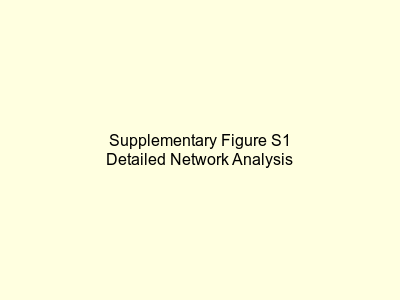
\includegraphics[width=0.8\textwidth]{supplementary/SupplementaryFigure1.png}
    \caption{Detailed build process flowchart showing the three-pass LaTeX compilation, bibliography processing, and final PDF generation stages.}
    \label{fig:supp1}
\end{figure}

\subsection{Customization Guidelines}

The template can be customized for different publication requirements by modifying the document class parameters and style definitions while maintaining compatibility with the automated build system.
